\let\negmedspace\undefined
\let\negthickspace\undefined
\documentclass[journal]{IEEEtran}
\usepackage[a4paper, margin=10mm, onecolumn]{geometry}
%\usepackage{lmodern} % Ensure lmodern is loaded for pdflatex
\usepackage{tfrupee} % Include tfrupee package

\setlength{\headheight}{1cm} % Set the height of the header box
\setlength{\headsep}{0mm}  % Set the distance between the header box and the top of the text

\usepackage{gvv-book}
\usepackage{gvv}
\usepackage{cite}
\usepackage{amsmath,amssymb,amsfonts,amsthm}
\usepackage{algorithmic}
\usepackage{graphicx}
\usepackage{float}
\usepackage{textcomp}
\usepackage{xcolor}
\usepackage{txfonts}
\usepackage{listings}
\usepackage{enumitem}
\usepackage{mathtools}
\usepackage{gensymb}
\usepackage{comment}
\usepackage[breaklinks=true]{hyperref}
\usepackage{tkz-euclide} 
\usepackage{listings}
% \usepackage{gvv}                                        
\def\inputGnumericTable{}                                 
\usepackage[latin1]{inputenc}                                
\usepackage{color}                                            
\usepackage{array}                                            
\usepackage{longtable}                                       
\usepackage{calc}                                             
\usepackage{multirow}                                         
\usepackage{hhline}                                           
\usepackage{ifthen}                                           
\usepackage{lscape}
\usepackage{tikz}
\usetikzlibrary{patterns}

\begin{document}

\bibliographystyle{IEEEtran}
\vspace{3cm}

\title{9.7.7}
\author{ee25btech11063-vejith}

\maketitle
% \maketitle
% \newpage
% \bigskip
{\let\newpage\relax\maketitle}
\renewcommand{\thefigure}{\theenumi}
\renewcommand{\thetable}{\theenumi}
\setlength{\intextsep}{10pt} % Space between text and floats
\textbf{Question}\\
\text{Find the solution of the pair of equations:} \quad 
$\frac{3}{x} + \frac{8}{y} = -1, 
\qquad 
\frac{1}{x} - \frac{2}{y} = 2, 
\qquad x,y \neq 0.$\\
\textbf{Solution}:\\
let 
\begin{align}
    \frac{1}{x}=u\\
    \frac{1}{y}=v\\
    \implies 3u+8v=-1\\
    u-2v=2
\end{align}
Equations (3) and (4) cann be written as
\begin{align}
    \begin{pmatrix}
        3 & 8\\
        1 & -2
    \end{pmatrix}\myvec{u\\v}=\myvec{-1\\2}
\end{align}
Forming the augmented matrix
\begin{align}
    \implies 
\left(\begin{array}{cc|c}
        3 & 8 & -1 \\
        1 & -2 & 2 
\end{array}\right) 
\xleftrightarrow{R_2 \rightarrow R_2-\frac{1}{3} \times R_1} \left(\begin{array}{cc|c}
        3 & 8 & -1 \\
        0 & -\frac{14}{3} & \frac{7}{3} 
\end{array}\right) 
\end{align}
on back substitution we get 
\begin{align}
    \myvec{u\\v}=\myvec{1\\-\frac{1}{2}}
\end{align}
From (1) and (2) we get
\begin{align}
    \myvec{x\\y}=\myvec{1\\-2}
\end{align}
\begin{figure}
    \centering
    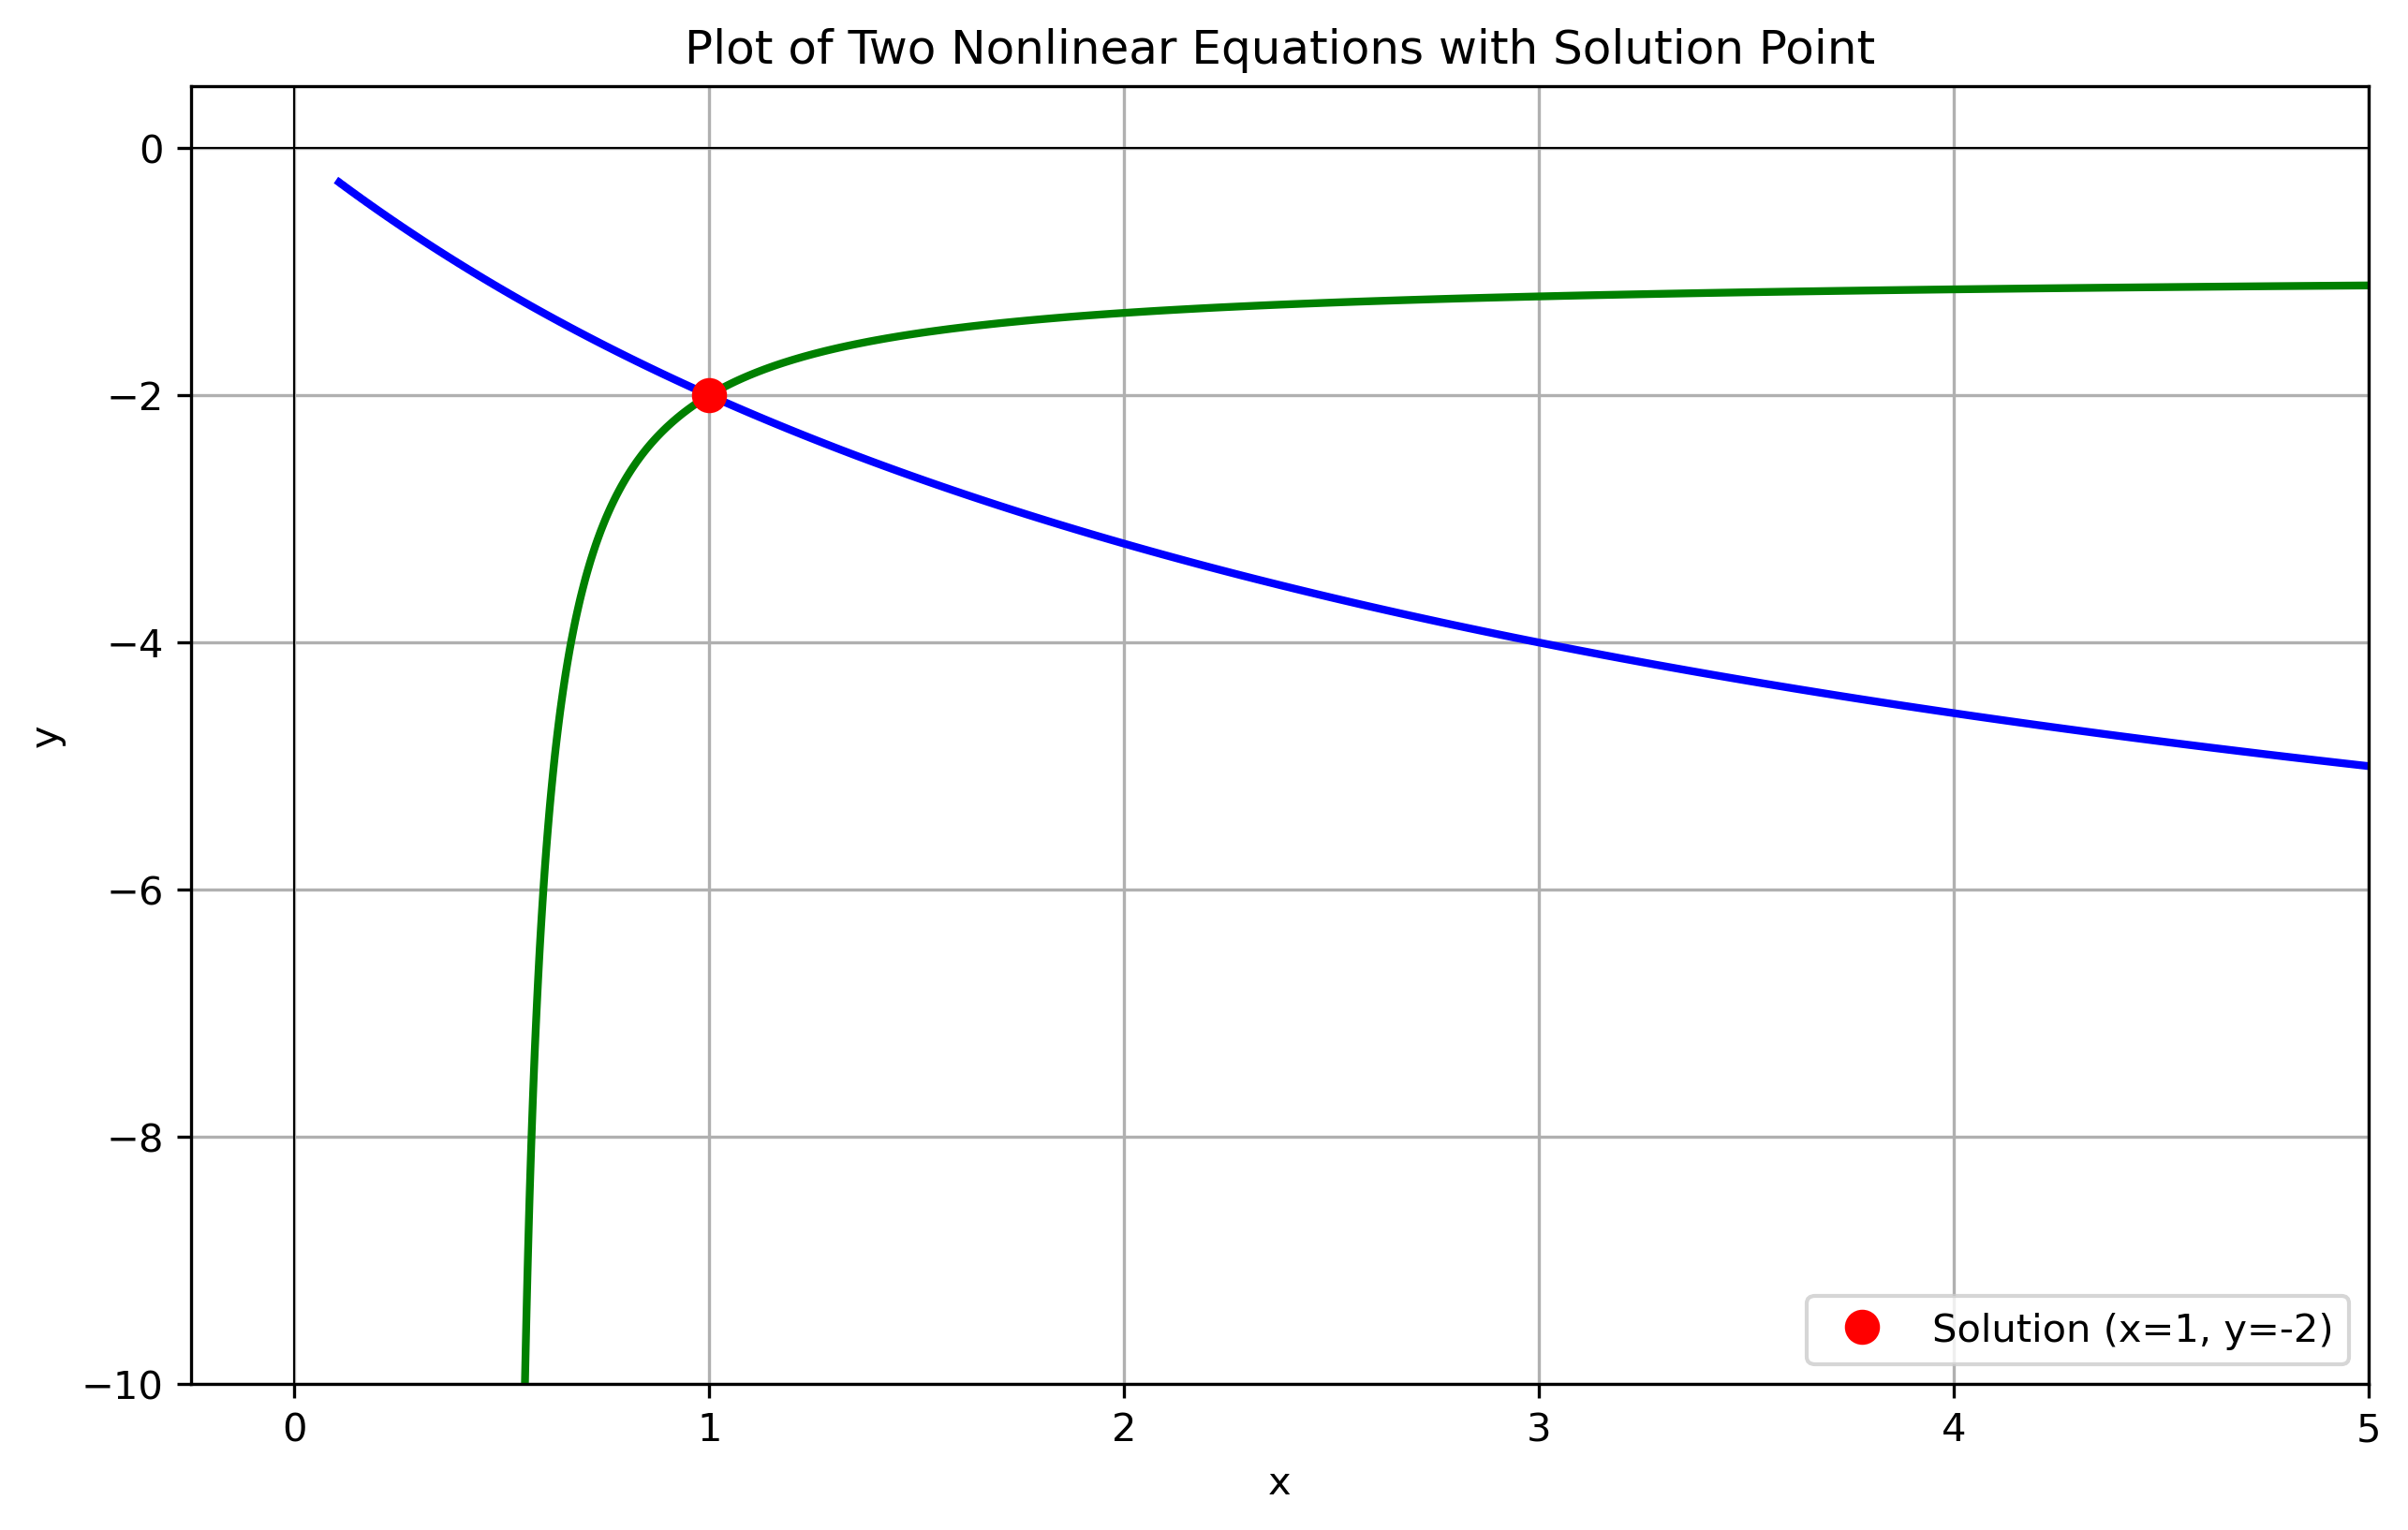
\includegraphics[width=0.85\columnwidth]{figs/01.png}
    \caption{}
    \label{fig:placeholder}
\end{figure}
\end{document}
